%%--- Set figure directory
%\inputdir{../ch2/comp}
\documentclass[xcolor=dvipsnames,notes]{beamer}
\usecolortheme[named=Brown]{structure}
\usetheme{default}
\setbeamertemplate{navigation symbols}{} 
\usepackage{tikz}
\usetikzlibrary{arrows,decorations.pathmorphing,backgrounds,positioning,fit}
\usetikzlibrary{datavisualization.formats.functions}
\usetikzlibrary{shapes}
%     
%Here are some macro's saving time and labour:     
%     
\newcommand{\const}{\mbox{const}}      
\newcommand{\est}{\mbox{{\tiny est}}}      
\newcommand{\im}{\mbox{$\Im \mbox{m}$}}      
\newcommand{\obs}{\mbox{{\tiny obs}}}      
\newcommand{\otherwise}{\mbox{otherwise}}      
\newcommand{\real}{\mbox{$\Re \mbox{e}$}}      
\newcommand{\sign}{\mbox{sign}}      
\newcommand{\sinc}{\mbox{sinc}}      
%
\newcommand{\p}{\mbox{$\partial$}}      
\renewcommand{\d}{\mbox{$\partial$}}      
\newcommand{\w}{\mbox{$\omega$}}      
%
\newcommand{\AAA}{\mbox{\boldmath $A$}}   
\newcommand{\BB}{\mbox{\boldmath $B$}}     
\newcommand{\CC}{\mbox{\boldmath $C$}}     
\newcommand{\DD}{\mbox{\boldmath $D$}}     
\newcommand{\EE}{\mbox{\boldmath $E$}}     
\newcommand{\FF}{\mbox{\boldmath $F$}}   
\newcommand{\GG}{\mbox{\boldmath $G$}}   
\newcommand{\HH}{\mbox{\boldmath $H$}}   
\newcommand{\II}{\mbox{\boldmath $I$}}   
\newcommand{\JJ}{\mbox{\boldmath $J$}}   
\newcommand{\KK}{\mbox{\boldmath $K$}}   
\newcommand{\LL}{\mbox{\boldmath $L$}}   
\newcommand{\MM}{\mbox{\boldmath $M$}}   
\newcommand{\NN}{\mbox{\boldmath $N$}}   
\newcommand{\OO}{\mbox{\boldmath $O$}}   
\newcommand{\PP}{\mbox{\boldmath $P$}}   
\newcommand{\QQ}{\mbox{\boldmath $Q$}}   
\newcommand{\RR}{\mbox{\boldmath $R$}}   
\newcommand{\SSS}{\mbox{\boldmath $S$}}   
\newcommand{\TT}{\mbox{\boldmath $T$}}   
\newcommand{\UU}{\mbox{\boldmath $U$}}   
\newcommand{\VV}{\mbox{\boldmath $V$}}   
\newcommand{\WW}{\mbox{\boldmath $W$}}   
\newcommand{\XX}{\mbox{\boldmath $X$}}   
\newcommand{\YY}{\mbox{\boldmath $Y$}}   
\newcommand{\ZZ}{\mbox{\boldmath $Z$}}   
%
%\newcommand{\aaa}{\mbox{\boldmath $a$}}     
\newcommand{\bb}{\mbox{\boldmath $b$}}     
\newcommand{\cc}{\mbox{\boldmath $c$}}     
\newcommand{\dd}{\mbox{\boldmath $d$}}     
\newcommand{\ee}{\mbox{\boldmath $e$}}   
\newcommand{\ff}{\mbox{\boldmath $f$}}   
%\newcommand{\ggg}{\mbox{\boldmath $g$}}   
\newcommand{\hh}{\mbox{\boldmath $h$}}   
\newcommand{\ii}{\mbox{\boldmath $i$}}   
\newcommand{\jj}{\mbox{\boldmath $j$}}   
\newcommand{\kk}{\mbox{\boldmath $k$}}   
%\newcommand{\lll}{\mbox{\boldmath $l$}}   
\newcommand{\mm}{\mbox{\boldmath $m$}}   
\newcommand{\nn}{\mbox{\boldmath $n$}}   
\newcommand{\pp}{\mbox{\boldmath $p$}}   
\newcommand{\qq}{\mbox{\boldmath $q$}}   
\newcommand{\rr}{\mbox{\boldmath $r$}}   
%\newcommand{\sss}{\mbox{\boldmath $s$}}   
%\newcommand{\ttt}{\mbox{\boldmath $t$}}   
\newcommand{\uu}{\mbox{\boldmath $u$}}   
\newcommand{\vv}{\mbox{\boldmath $v$}}   
\newcommand{\ww}{\mbox{\boldmath $w$}}   
\newcommand{\xx}{\mbox{\boldmath $x$}}   
\newcommand{\yy}{\mbox{\boldmath $y$}}   
\newcommand{\zz}{\mbox{\boldmath $z$}}   
%
\newcommand{\balpha}{\mbox{\boldmath $\alpha$}}     
\newcommand{\bpsi}{\mbox{\boldmath $\psi$}}     
\newcommand{\bphi}{\mbox{\boldmath $\phi$}}     
\newcommand{\bbeta}{\mbox{\boldmath $\beta$}}     
\newcommand{\btheta}{\mbox{\boldmath $\theta$}}     
\newcommand{\bdelta}{\mbox{\boldmath $\delta$}}     
\newcommand{\bgamma}{\mbox{\boldmath $d$}}     
\newcommand{\bGamma}{\mbox{\boldmath $\Gamma$}}     
\newcommand{\bLambda}{\mbox{\boldmath $\Lambda$}}     
\newcommand{\bmu}{\mbox{\boldmath $\mu$}}     
\newcommand{\bnabla}{\mbox{\boldmath $\nabla$}}     
\newcommand{\brho}{\mbox{\boldmath $\rho$}}     
\newcommand{\bSigma}{\mbox{\boldmath $\Sigma$}}     
\newcommand{\bsigma}{\mbox{\boldmath $\sigma$}}     
\newcommand{\bxi}{\mbox{\boldmath $\xi$}}     
\newcommand{\bepsilon}{\mbox{\boldmath $\epsilon$}}     
\newcommand{\blambda}{\mbox{\boldmath $\lambda$}}     
\newcommand{\BLambda}{\mbox{\boldmath $\Lambda$}}     
%-------------------------------------%
%  \Appendix - a new appendix command %
%-------------------------------------%
%The appendix command is used as in
% \Appendix{A}{The wave equation as a matrix equation}
\newcommand {\Appendix}[1]{
              \section*{APPENDIX #1}
              \setcounter{equation}{0}
              \renewcommand{\theequation} 
              {A-\arabic{equation}}}
\newcommand {\Appendices}[2]{
              \section*{APPENDIX #1: #2 }
              \setcounter{equation}{0}
              \renewcommand{\theequation} 
              {#1-\arabic{equation}}}
%------------------------------------%
%    \aref - a new cite command.     % 
%------------------------------------%
\newcommand{\aref}[2]{\nocite{#1}#2} 
%----------------------------------------
%\eqref -an equation reference command
%----------------------------------------
%\newcommand{\eqref}[1]{(\ref{#1})}
%\newcommand{\eqref}[1]{\ref{#1}}

\usepackage{epsfig}
\usepackage{natbib}
\usepackage{graphicx}
\usepackage{multimedia}
\begin{document}
%\setbeamercolor{titlelike}{fg=gray,bg=white}
%\setbeamercolor{itemize item}{fg=gray,bg=white}
%\setbeamercolor{enumerate item}{fg=gray,bg=white}
%\setbeamercolor{block title}{fg=black,bg=white}
%==============================================
\title{TPG4190 Seismic data acquisition and processing \\
               Lecture 4: Fourier Transforms}
\author{B. Arntsen}
\institute[NTNU]{
  NTNU\\
  Department of Geoscience and petroleum \\
  \texttt{borge.arntsen@ntnu.no}
}
\date{Trondheim fall 2021}
\begin{frame}
 \titlepage
\end{frame}
%==============================================
\begin{frame}{Overview}
%==============================================
\begin{itemize}
  \item The Fourier Transform
  \end{itemize}
\end{frame}
%==============================================
\begin{frame}{The Continous Fourier Transform}
%==============================================
The Fourier transform $A(f)$ of a time signal $a(t)$ is defined as
%
\begin{eqnarray}
 A(f) = \int^{+\infty}_{-\infty} dt\, a(t) \exp(-2\pi i f t) \label{eq:2-ft},
\end{eqnarray}
%
with the inverse transform given as
%
\begin{eqnarray}
 a(t) = \int^{+\infty}_{-\infty} df\, A(f) \exp(2\pi i f t) \label{eq:2-ift}.
\end{eqnarray}
%
Here $t$ is time and $f$ is frequency.
\end{frame}
%==============================================
\begin{frame}{The Continous Fourier Transform}
%==============================================
Angular frequency $\omega=2\pi f$is often used instead
of the frequency, so that equations \eqref{eq:2-ft} and \eqref{eq:2-ift} becomes
%
\begin{eqnarray}
 a(t) = \frac{1}{2\pi}\int^{+\infty}_{-\infty} d\omega\, A(\omega) \exp(i\omega t),\label{eq:2-ftb}\\
 A(\omega) = \int^{+\infty}_{-\infty} dt\, a(t) \exp(-i\omega t) \label{eq:2-iftb}.
\end{eqnarray}
%
\end{frame}
%==============================================
\begin{frame}{Amplitude and phase}
%==============================================
We now introduce the concepts  {\em Amplitude spectrum} and
{\em Phase spectrum}. 
%
\begin{eqnarray}
  A(f) = |A(f)|\exp[i\phi(f)],
  \label{eq:2-70}
\end{eqnarray}
%
where
%
\begin{eqnarray}
  |A(f)| = \sqrt{A^*(f) A(f)},
  \label{eq:2-71}
\end{eqnarray}
%
and
%
\begin{eqnarray}
  \tan[\phi(f)] = \mbox{Im}[A(f)]/\mbox{Re}[A(f)].
  \label{eq:2-72}
\end{eqnarray}
%
$|A(f)|=\sqrt{A^*(f)A(f)}$ is called the amplitude spectrum,
while the phase spectrum (or just the phase for short) is defined by
$\phi(f) = \tan^{-1}[Im(A(f)]/Re[A(f)]$.
\end{frame}
%==============================================
\begin{frame}{The Fourier transforms of a constant}
%==============================================
%
\begin{eqnarray}
 a(t)=c,
\end{eqnarray}
where $c$ is a constant.
Inserting the equation above into \eqref{eq:2-ift} we get
%
\begin{eqnarray}
A(f) = \int^{+\infty}_{-\infty} dt\, c \exp(-2\pi i f t), 
\end{eqnarray}
%
and because $c$ is a constant we get
%
\begin{eqnarray}
A(f) = c\int^{+\infty}_{-\infty} dt\, \exp(-2\pi i f t). 
  \label{eq:2-720}
\end{eqnarray}
%
\end{frame}
%==============================================
\begin{frame}{The $\delta$ - function}
%==============================================
Before we can proceed we need to introduce the delta function, defined by
\begin{eqnarray}
f(0)=\int^{+\infty}_{-\infty}dt\ f(t)\delta(t).
\end{eqnarray}
The Fourier transform of a $\delta$-function
%
\begin{eqnarray}
a(t)=1 = \int^{+\infty}_{-\infty} df\, \delta(f)\exp(2\pi i ft),
  \label{eq:2-idelta}
\end{eqnarray}
and hence
%
\begin{eqnarray}
\delta(f)= \int^{+\infty}_{-\infty} dt\, \exp(-2\pi i ft),
  \label{eq:2-idelta}
\end{eqnarray}

%
\end{frame}
%==================================================
\begin{frame}{The Fourier transform of a constant}
%==================================================

By using the delta function we see that that equation \eqref{eq:2-720} is equal to
%
\begin{eqnarray}
A(f) = c\delta(f).
  \label{eq:2-721}
\end{eqnarray}
%
The Fourier transform of a constant is a delta function at zero frequency. 
\end{frame}
%==================================================
\begin{frame}{The Fourier transforms of a boxcar}
%==================================================
Another Fourier transform which will turn out to be usefull, is the case of a boxcar function defined by:
%
\begin{eqnarray}
h(t)=\left\{ \begin{array}{ll}
                        1  & \mbox{if $|t| <  L/2$}  \\
                        0  & \mbox{otherwise}
             \end{array}
     \right.             
     \label{eq:2-722}
\end{eqnarray}
Inserting equation \eqref{eq:2-722} into \eqref{eq:2-ift} we get
%
\begin{eqnarray}
A(f) = \int^{+L/2}_{-L/2} dt\,  \exp(-2\pi i f t), 
\end{eqnarray}
%
which can be integrated to give
%
\begin{eqnarray}
A(f) = |^{+L/2}_{-L/2} dt\,  \frac{\exp(-2\pi i f t)}{-2\pi i f}. 
\end{eqnarray}
%
\end{frame}
%==================================================
\begin{frame}{The Fourier transforms of a boxcar}
%==================================================
Inserting the upper and lower limits this is equal to
%
\begin{eqnarray}
A(f) =  \frac{\exp(\pi i f L)-\exp(-\pi i f L)}{2\pi i f}. 
            \label{eq:2-723}
\end{eqnarray}
%
By using the identity
%
\begin{eqnarray}
 \sin(x)=\frac{\exp(ix)-\exp(-ix)}{2i},
\end{eqnarray}
equation \eqref{eq:2-723} becomes
%
\begin{eqnarray}
A(f) =  \frac{\sin(\pi f L)}{\pi f}, 
            \label{eq:2-725}
\end{eqnarray}
which is finally rewritten to
%
\begin{eqnarray}
A(f) =  L \frac{\sin(\pi f L)}{\pi f L}. 
            \label{eq:2-726}
\end{eqnarray}
%
\end{frame}
%================================================================
\begin{frame}{The Fourier transforms of a time-delayed function}
%=================================================================
%
Consider the function $a(t-\tau)$, where $\tau$ is a constant time delay. Inserting this
function into \eqref{eq:2-ift} we get
%
\begin{eqnarray}
A(f) = \int^{+\infty}_{-\infty} dt\, a(t-\tau) \exp(-2\pi i f t). 
\end{eqnarray}
%
Change of variable $u=t-\tau$ and observing $t=u+\tau$
%
\begin{eqnarray}
A(f) = \int^{+\infty}_{-\infty} du\, a(u) \exp[-2\pi i f (u+\tau)], 
\end{eqnarray}
%
which is equal to
%
\begin{eqnarray}
A(f) = \exp(-2\pi i f \tau) \int^{+\infty}_{-\infty} du\, a(u) \exp(-2\pi i f u). 
\end{eqnarray}
%
Which implies that a delay of $\tau$ leads to a change in the phase of the Fourier transform
by $-2\pi i f \tau$.
\end{frame}
%================================================================
\begin{frame}{The Fourier transforms of a derivative}
%=================================================================
The Fourier transform of the derivative of a function can be calculated by taking the derivative
of both sides of equation \eqref{eq:2-ftb} 
\begin{eqnarray}
 \frac{d a(t)}{dt} = a'(t)=\frac{1}{2\pi}\int^{+\infty}_{-\infty} d\omega\, i\omega A(\omega) \exp(i\omega t)
\end{eqnarray}
Compar with the definition of the inverse Fourier transform,\eqref{eq:2-ftb}, we
conclude that the Fourier transform of $a'(t)$ has to be equal to $i\omega A(\omega)$. 
\end{frame}

%================================================================
\begin{frame}{The Fourier transforms of the convolution integral}
%=================================================================
The convolution integral is defined by
\begin{eqnarray}
a(t)=\int^{+\infty}_{-\infty} d\tau s(t-\tau)h(\tau),
\end{eqnarray}
where $s$ and $h$ are arbitrary functions.

A very important property of convolution is that it can be expressed as
an operation on the Fourier transforms of $s(t)$ and $h(t)$.
Assume that the Fourier transforms of $s(t)$ and $h(t)$ are given by
%
\begin{eqnarray}
 S(f) = \int^{+\infty}_{-\infty} dt\, s(t) 
      \exp(-2\pi i f t) ,\\
 H(f) = \int^{+\infty}_{-\infty} dt\, h(t) 
      \exp(-2\pi i f t).
\end{eqnarray}
%
\end{frame}
%================================================================
\begin{frame}{The Fourier transforms of the convolution integral}
%=================================================================
The Fourier transform of the convolution of $h(t)$ and $s(t)$ is
%
\begin{eqnarray}
 \int^{+\infty}_{-\infty}dt\, 
\int^{+\infty}_{-\infty}d\tau\, s(\tau) h(t-\tau)\exp(-2\pi i f t),
\end{eqnarray}
%
with the change of variable $u=t-\tau$, one gets 
%
\begin{eqnarray}
 \int^{+\infty}_{-\infty}du\, 
\int^{+\infty}_{-\infty}d\tau\, s(\tau) h(u)\exp[-2\pi i f (u+\tau)],
\end{eqnarray}
%
\end{frame}
%================================================================
\begin{frame}{The Fourier transforms of the convolution integral}
%=================================================================
which is
%
\begin{eqnarray}
 \int^{+\infty}_{-\infty}du\, h(u)\exp(-2\pi i f u)
\int^{+\infty}_{-\infty}d\tau\, s(\tau) \exp(-2\pi i f \tau).
   \label{eq:3-10} 
\end{eqnarray}
%
We recognize equation \eqref{eq:3-10} as
%
\begin{eqnarray}
  H(f) S(f).
   \label{eq:3-11} 
\end{eqnarray}
\end{frame}
%================================================================
\begin{frame}{The Fourier transforms of the convolution integral}
%=================================================================

We have established that the convolution of two functions 
%
\begin{eqnarray}
  g(t)=h(t)*s(t),
   \label{eq:3-12} 
\end{eqnarray}
%
corresponds to the product of the two functions after a Fourier
transform
%
\begin{eqnarray}
  G(f)=H(f)S(f).
   \label{eq:3-13} 
\end{eqnarray}
\end{frame}
%================================================================
\begin{frame}{The Discrete Fourier Transform}
%=================================================================
In acquisition of seismic data we deal with sampled 
time functions instead of continuous time functions.

A sampled time function is known only at a finite number
of time instances. If $a(t)$ is a continuous time function
defined on the interval $(0,T)$, a corresponding sampled time function $a_k$ is given by
%
\begin{eqnarray}
  a_k = a(k\Delta t), k=0,...,N
    \label{eq:2-17}
\end{eqnarray}
where 
\begin{itemize}
\item $\Delta t$: time sampling interval 
\item $N$:  $N=T/\Delta t $.
\end{itemize}
\end{frame}
%================================================================
\begin{frame}{The Discrete Fourier Transform}
%=================================================================
Key questions: 
\begin{itemize}
\item Is it possible to
recover the continuous function $a(t)$ from the samples given by $a_k$? 
\item
What (if any) are the requirements on $a(t)$ and how should the sampling interval
$\Delta t$ be chosen?
\end{itemize}
\end{frame}
%================================================================
\begin{frame}{The Discrete Fourier Transform}
%=================================================================
%
\begin{figure}
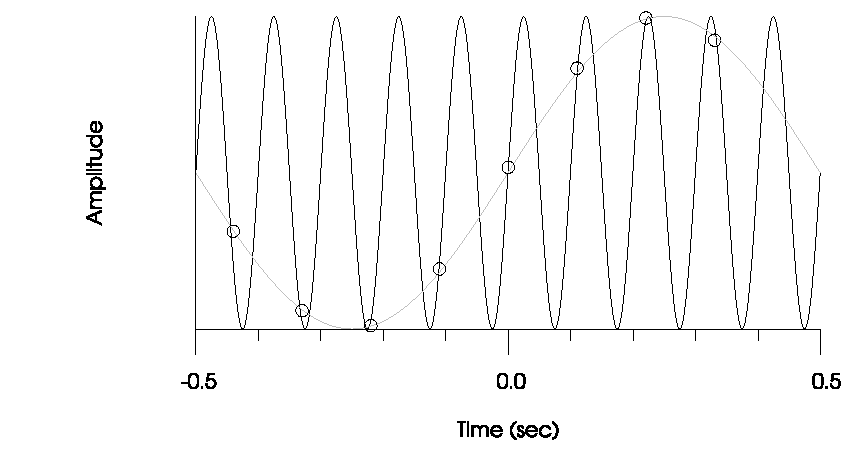
\includegraphics{Fig/alias.pdf}
\end{figure}
%
\end{frame}
%================================================================
\begin{frame}{The Discrete Fourier Transform}
%=================================================================
The discrete analogue of the continuous Fourier transform is defined by the equations
%
\begin{eqnarray}
  A_n   &=& \frac{1}{N}\sum^{N-1}_{k=0} a_k\exp(-2\pi i n k/N),
    \label{eq:2-66}
\end{eqnarray}
%
and the inverse transform
%
\begin{eqnarray}
  a_k   &=& \sum^{N-1}_{n=0} A_n\exp(2\pi i n k /N).
    \label{eq:2-67}
\end{eqnarray}
%
\end{frame}
%================================================================
\begin{frame}{The Discrete Fourier Transform}
%=================================================================
Here $A_n$ correspond to $A(f)$.
The frequency, $f$, is now discrete and related to the time period $T$ through
\begin{eqnarray}
f_n=n/T
\end{eqnarray}.
We also have that the frequency sampling interval $\Delta f=f_{n+1}-f_{n}$ is given
by
\begin{eqnarray}
 \Delta f = 1/T.
\end{eqnarray}

Equations \eqref{eq:2-66} and \eqref{eq:2-67} are the standard formulation
of the Discrete Fourier Transform (DFT). 
\end{frame}
%================================================================
\begin{frame}{The Discrete Fourier Transform}
%=================================================================
The DFT is periodic with period N, 
\begin{eqnarray}
A_{N+l}=A_l,
\end{eqnarray}
which can be seen by setting $n=N+l$ in equation
\eqref{eq:2-66}:
%
\begin{eqnarray}
  A_{N+l}   &=& \frac{1}{N}\sum^{N-1}_{k=0} a_k\exp[-2\pi i (N+l) k/N],\nonumber\\
  A_{N+l}   &=& \frac{1}{N}\sum^{N-1}_{k=0} a_k\exp(-2\pi i k)\exp[(-2\pi i lk)/N] \nonumber\\,
            &=&A_l
    \label{eq:dft-period}
\end{eqnarray}
%
because $\exp(-2\pi i k)=cos(2\pi k)+i\sin(2\pi k)=1$ for integer values of $k$.
\end{frame}
%================================================================
\begin{frame}{The Discrete Fourier Transform}
%=================================================================
Another important property follows from the fact that $a(t)$ must always be real.
Taking the complex conjugate of equation \eqref{eq:2-66} one gets
%
\begin{eqnarray}
  A^*_n   &=& \frac{1}{N}\sum^{N-1}_{k=0} a_k\exp(2\pi i n k/N), \nonumber\\
  A^*_n   &=& \frac{1}{N}\sum^{N-1}_{k=0} a_k\exp[-2\pi i (-n) k/N], \nonumber\\
          &=& A_{-n}
\end{eqnarray}
%
which implies
\begin{eqnarray}
A_{-n}=A^*.
\label{eq:dft-conjg}
\end{eqnarray}

An immediate implication is that
\begin{eqnarray}
A^*_0 = A_0,
\end{eqnarray}
hence the zero-frequency value is always real.
\end{frame}
%================================================================
\begin{frame}{The Fast Fourier Transform}
%=================================================================

A particular efficient implementation of the DFT is known
as the Fast Fourier Transform (FFT). The FFT is in practice used instead
of the DFT for numerical work. 
\begin{itemize}
  \item Compute time for DFT is proportional to $N^2$
  \item Compute time for FFT is proportional to $N\log N$
\end{itemize}
\end{frame}
%================================================================
\begin{frame}{Aliasing}
%=================================================================
Equation \eqref{eq:dft-conjg} implies that the spectrum is symmetric around $n=0$
\begin{eqnarray}
|A_n|=|A_{-n}|,
\end{eqnarray}
and since $A_n$ is periodic with peeriod $N$ it implies that $A_n$ is unique only for
values of $|n| \leq N/2$. In other words, if the Discrete Fourier Transform is going to
be used to yield a unique transform we must demand tha
%
\begin{eqnarray}
  A_{n} = 0 \quad \mbox{for} |n|> N/2.  
\end{eqnarray}
%
This implies that there exist a largest frequency, the Nyquist frequency, given by
%
\begin{eqnarray}
  f_{Nyq}=\Delta f N/2 = \frac{N}{2T},
\end{eqnarray}
which is equal to
\begin{eqnarray}
 f_{Nyq}= \frac{1}{2\Delta t}.
\label{eq:fnyq}
\end{eqnarray}
\end{frame}
%================================================================
\begin{frame}{The Nyquist limit}
%=================================================================
%
\begin{eqnarray}
  f \leq  \frac{1}{2\Delta t}.
\label{eq:nyqcond}
\end{eqnarray}
%
\end{frame}
%================================================================
\begin{frame}{Aliasing}
%=================================================================
True (continous) amplitude spectrum
\begin{figure}
\begin{tikzpicture}
  \draw[->] (0,0) -- (5,0) ; %Draw x-axis
  \draw[->] (0,0) -- (-5,0) ; %Draw x-axis
  \draw[->] (0,0) -- (0,4)  ; %Draw y-axis
  \draw (-5,0) node[below]{$-f$}; %Annotation negative x-axis
  \draw (-2,0) node[below]{$-f_{max}$}; %Annotation negative x-axis
  \draw (5,0) node[below]{$f$};   %Annotation positive x-axis
  \draw (2,0) node[below]{$f_{max}$};   %Annotation positive x-axis

  \draw (0,0) -- (1,2)  ; %Draw positive spectrum 1
  \draw (1,2) -- (2,0)  ; %Draw positive spectrum 1
  
  %\draw (2,0) -- (3,2)  ; %Draw positive spectrum 2
  %\draw (3,2) -- (4,0)  ; %Draw positive spectrum 2

  %\draw (4,0) -- (5,2)  ; %Draw positive half spectrum 2

  \draw (0,0) -- (-1,2)  ; %Draw negative spectrum 1
  \draw (-1,2) -- (-2,0) ; %Draw negative spectrum 1
  
  %\draw (-2,0) -- (-3,2)  ; %Draw negative spectrum 2
  %\draw (-3,2) -- (-4,0)  ; %Draw negative spectrum 2

  %\draw (-4,0) -- (-5,2)  ; %Draw negative half spectrum 2

  %\draw[<-] (0.1,2.5) -- (1.6,2.5); %Draw left arrow   
  %\draw[->] (2.4,2.5) -- (4,2.5); %Draw right arrow
  %\draw (2.0,2.5) node{$N$} ;     %Draw N/2
\end{tikzpicture}
\label{fig:cont}
\end{figure}
\end{frame}
%================================================================
\begin{frame}{Aliasing}
%=================================================================
Spectrum of sampled function
\begin{figure}
\begin{tikzpicture}
  \draw[->] (0,0) -- (5,0) ; %Draw x-axis
  \draw[->] (0,0) -- (-5,0) ; %Draw x-axis
  \draw[->] (0,0) -- (0,4)  ; %Draw y-axis
  \draw (-5,0) node[below]{$-f$}; %Annotation negative x-axis
  \draw (-2,0) node[below]{$-f_{max}$}; %Annotation negative x-axis
  \draw (5,0) node[below]{$f$};   %Annotation positive x-axis
  \draw (2,0) node[below]{$f_{max}$};   %Annotation positive x-axis

  \draw (0,0) -- (1,2)  ; %Draw positive spectrum 1
  \draw (1,2) -- (2,0)  ; %Draw positive spectrum 1
  
  \draw (2,0) -- (3,2)  ; %Draw positive spectrum 2
  \draw (3,2) -- (4,0)  ; %Draw positive spectrum 2

  \draw (4,0) -- (5,2)  ; %Draw positive half spectrum 2

  \draw (0,0) -- (-1,2)  ; %Draw negative spectrum 1
  \draw (-1,2) -- (-2,0) ; %Draw positive spectrum 1
  
  \draw (-2,0) -- (-3,2)  ; %Draw negative spectrum 1
  \draw (-3,2) -- (-4,0)  ; %Draw negative spectrum 1

  \draw (-4,0) -- (-5,2)  ; %Draw negative half spectrum 2

  \draw[<-] (0.1,2.5) -- (1.6,2.5); %Draw left arrow   
  \draw[->] (2.4,2.5) -- (4,2.5); %Draw right arrow
  \draw (2.0,2.5) node{$N$} ;     %Draw N/2
\end{tikzpicture}
\label{fig:aliasing}
\end{figure}
\end{frame}
%================================================================
\begin{frame}{Aliasing}
%=================================================================
Spectrum of incorrectly sampled function
\begin{figure}
\begin{tikzpicture}
  \draw[->] (0,0) -- (5.25,0) ; %Draw x-axis
  \draw[->] (0,0) -- (-5.25,0) ; %Draw x-axis
  \draw[->] (0,0) -- (0,4)  ; %Draw y-axis
  \draw (-5,0) node[below]{$-f$}; %Annotation negative x-axis
  \draw (-2,0) node[below]{$-f_{max}$}; %Annotation negative x-axis
  \draw[dashed] (-2,0) -- (-2.0,0.7) ;
  \draw (5,0) node[below]{$f$};   %Annotation positive x-axis
  \draw[dashed] (2.,0) -- (2.0,0.7) ;
  \draw (2,0) node[below]{$f_{max}$};   %Annotation positive x-axis

  \draw (0,0) -- (1,2)  ; Draw positive spectrum 1
  \draw (1,2) -- (2,0)  ; Draw positive spectrum 1
  \draw (1.75,0) -- (2.75,2)  ; Draw positive spectrum 2
  \draw (2.75,2) -- (3.75,0)  ; Draw positive spectrum 2
  \draw (3.75,0) -- (4.75,2)  ; Draw positive half spectrum 2

  \draw (0,0) -- (-1,2)  ; Draw positive spectrum 1
  \draw (-1,2) -- (-2,0)  ; Draw positive spectrum 1
  \draw (-1.75,0) -- (-2.75,2)  ; Draw positive spectrum 2
  \draw (-2.75,2) -- (-3.75,0)  ; Draw positive spectrum 2
  \draw (-3.75,0) -- (-4.75,2)  ; Draw positive half spectrum 2

  \draw[<-] (0.1,2.5) -- (1.5,2.5); %Draw left arrow   
  \draw[->] (2.4,2.5) -- (3.75,2.5); %Draw right arrow
  \draw (2.0,2.5) node{$L$} ;     %Draw L
\end{tikzpicture}
\label{fig:aliasing2}
\end{figure}
\end{frame}
%================================================================
\begin{frame}{Discrete Fourier Transform}
%=================================================================
\begin{figure}
  \setlength{\unitlength}{0.6mm}
\begin{picture}(150,100)
  \put(0,20){\line(1,0){150}}
  \put(25,20){\line(0,1){60}}
  \put(25,0){$0$}
  \put(15,95){$f=0$}
  \put(75,20){\vector(0,1){70}}
  \put(60,95){$f=f_{Nyq}$}
  \put(75,0){$N/2$}
  \put(25,80){\line(1,0){100}}
  \put(125,20){\line(0,1){60}}
  \put(110,95){$f=-\Delta f$}
  \put(125,0){$N-1$}
\end{picture}
\label{fig:dft-even}
\end{figure}
\end{frame}
\end{document}

%%%%%%%%%%%%%%%%
%================================================================
\begin{frame}{Analysing noise}
%=================================================================
%
\plot{cos}{width=0.8\textwidth}{}
%
\end{frame}
%
%================================================================
\begin{frame}{Analysing noise}
%=================================================================
\plot{amp}{width=0.8\textwidth}{}
%
\end{frame}
%
%================================================================
\begin{frame}{Analysing noise}
%=================================================================
\plot{trace}{width=0.8\textwidth}{}
%
\end{frame}
%
%================================================================
\begin{frame}{Analysing noise}
%=================================================================
\plot{amp-trace}{width=0.8\textwidth}{}
%
\end{frame}
